%\section{Binary sensor imaging}
\subsection{Photon-Counting in Film Photography}

The principal notions of the single-bit imaging sensors can be traced back to analog photography and demonstrate behaviors reminiscent to ones of the silver halide emulsion, a common component in the photographic film. 

Akin to its digital counterpart, the photographic film is subjected to the photoelectric effect; in film, this is represented by the photographic emulsion coated on the transparent sheet of plastic. Such emulsion consists of microscopic crystals, or grains, of silver halides embedded in protective colloid like gelatin \cite{Carroll1980}, with the commonly considered compounds being silver bromide \textit{AgBr}, silver chloride \textit{AgCl}, silver iodide \textit{AgI}, or some mixture thereof \cite{Schroeder1981}.
%ionenbindung löst photographischen primärprozess: elektron durch quantenenergie abgespalten; wirkung des primproz ist srtreng proportional zu der quantenzahl!
\begin{figure}[h]
  \centering
  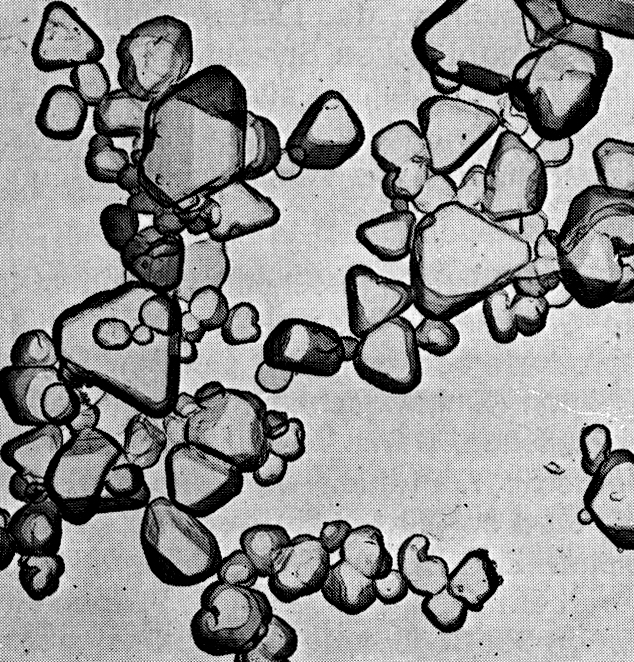
\includegraphics[width=0.5\linewidth]{imgs/film/silver.jpg}
  \caption{Electron microscopic structure of undeveloped silver bromide crystals, via \cite{AgfaABC}.}
  \label{fig:silverbromide}
  \Description{Small blackish crystals of silver on gray background}
\end{figure}

The process starts upon exposure of the film to the light. Film grains absorb the incoming radiation in form of the incident photons and dissociate into a group of free silver ions. 

Once exposed to development agent, the silver ions in the film are reduced to metallic silver, rendering the exposed regions of the film sheet opaque black. The unaltered halides are later dissolved out in a chemical bath, so that the corresponding spots are transparent. Each crystal can either be struck by a photon or not, and so the film exhibits a binary response. 

%chance of absorprtion of a photon by a grain; grain must absorb r quanta in order to be developable. when r = 1, equation is reduced to 1-e ^ (-q); the shape of the characteristic curve depends on photon distribution
The exposed grains are spread randomly, fluctuate in size and differ in absorption rate -- there is no uniformity regarding the required absorbed quanta as the particles arrive randomly. However, with the irradiance of the image areas varying, so does the stochastic photon distribution and therefore the concentration of silver particles per film area. 

Fine granular structures are not perceivable by the human eye and are registered as continuous tone of gray \cite{Feng_Yang_2012} instead, matching the overall area density to the original light intensity information; the mean number of absorbed quanta per grain is given by the Poisson equation. % (optical density)

%For conventional sensors some of this non-linear response can be encoded in the postprocessing of the linear-response image. Nevertheless, the non-linear response of film has been hard to match even in HDR solid-state image sensors without introducing artifacts due to motion, threshold voltage fixed- pattern variation, and other circuit design issues

\begin{figure}[h]
  \centering
  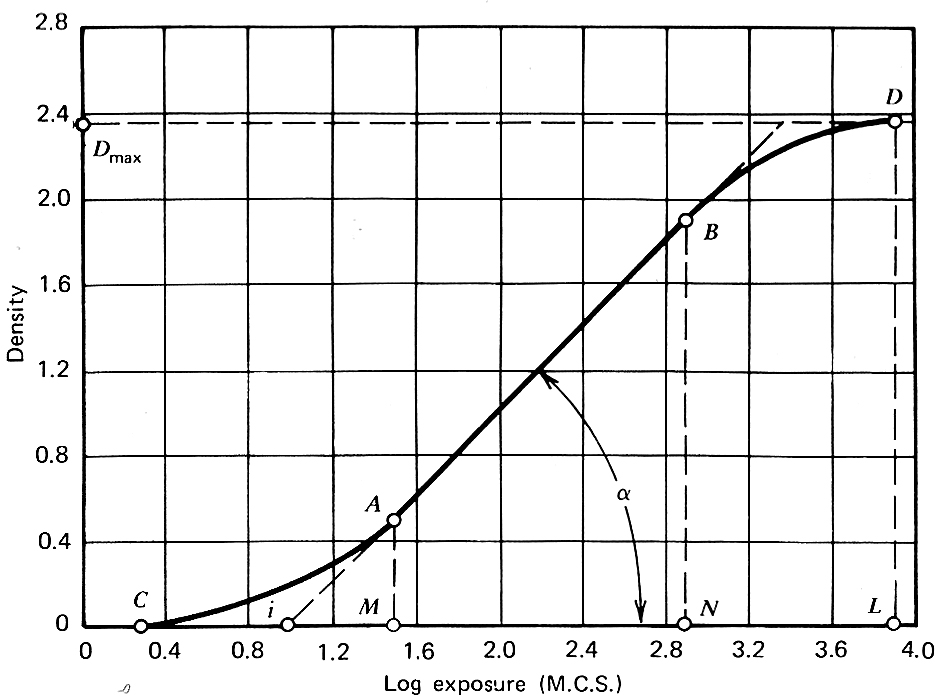
\includegraphics[width=\linewidth]{imgs/film/filmcurve.jpg}
  \caption{Exemplary characteristic curve of the film emulsion, via \cite{Saleh1991}.}
  \label{fig:filmcurve}
  \Description{S-shaped curve relates the optical density to the logarithmic exposure. There are two latitudes on both ends of the curve.}
\end{figure}
The photographic properties of the film emulsion are typically described through the ratio of the luminance transmitted in the medium to the luminance of the observed scene. The optical density is modelled as a function of logarithmic exposure and was first derived in \cite{HurterDriffield}. As seen in Figure \ref{fig:filmcurve}, this relationship has a non-linear behavior. 

The D - log H curve (also referred to as \textit{ characteristic curve}) can be split into three intervals based on the curvature of the response. For sufficiently small or large values of logH, the function is asymptotic and results in under- or overexposure (the toe and shoulder portions of the curve, respectively~\cite{Hunt2005}); in the middle interval, the slope is constant, and the relationship between the luminance and the photographic density is linear. %Under sparse exposures and overexposures, this means better tolerance for highlights
In general, the S-shape of the curve is determined by the underlying randomness of photon arrivals. (This is different in conventional CIS sensors.)

In film, the grains may fluctuate in size, ranging from 0.048 to 1.71 $\mu$m depending on the application; on average, one grain of the developed emulsion corresponds to ca. 3-4 electrons~\cite{Carroll1980, FossumSiMulQIS}. Feature sizes of QIS are similar in their capacitance; the jots in the single-carrier implementation of QIS are meant to store around 3 carriers as well. Thus, both digital sensors QIS and analog film deliver quantized, spatially discrete values obtained off similar area sizes. So, the behavior in binary imaging sensors is, too, dominated by the photon distribution. Resulting characteristic curve is shaped comparably, demonstrating slightly larger overexposure latitude~\cite{FossumSiMulQIS}.

\begin{figure}[h]
  \centering
  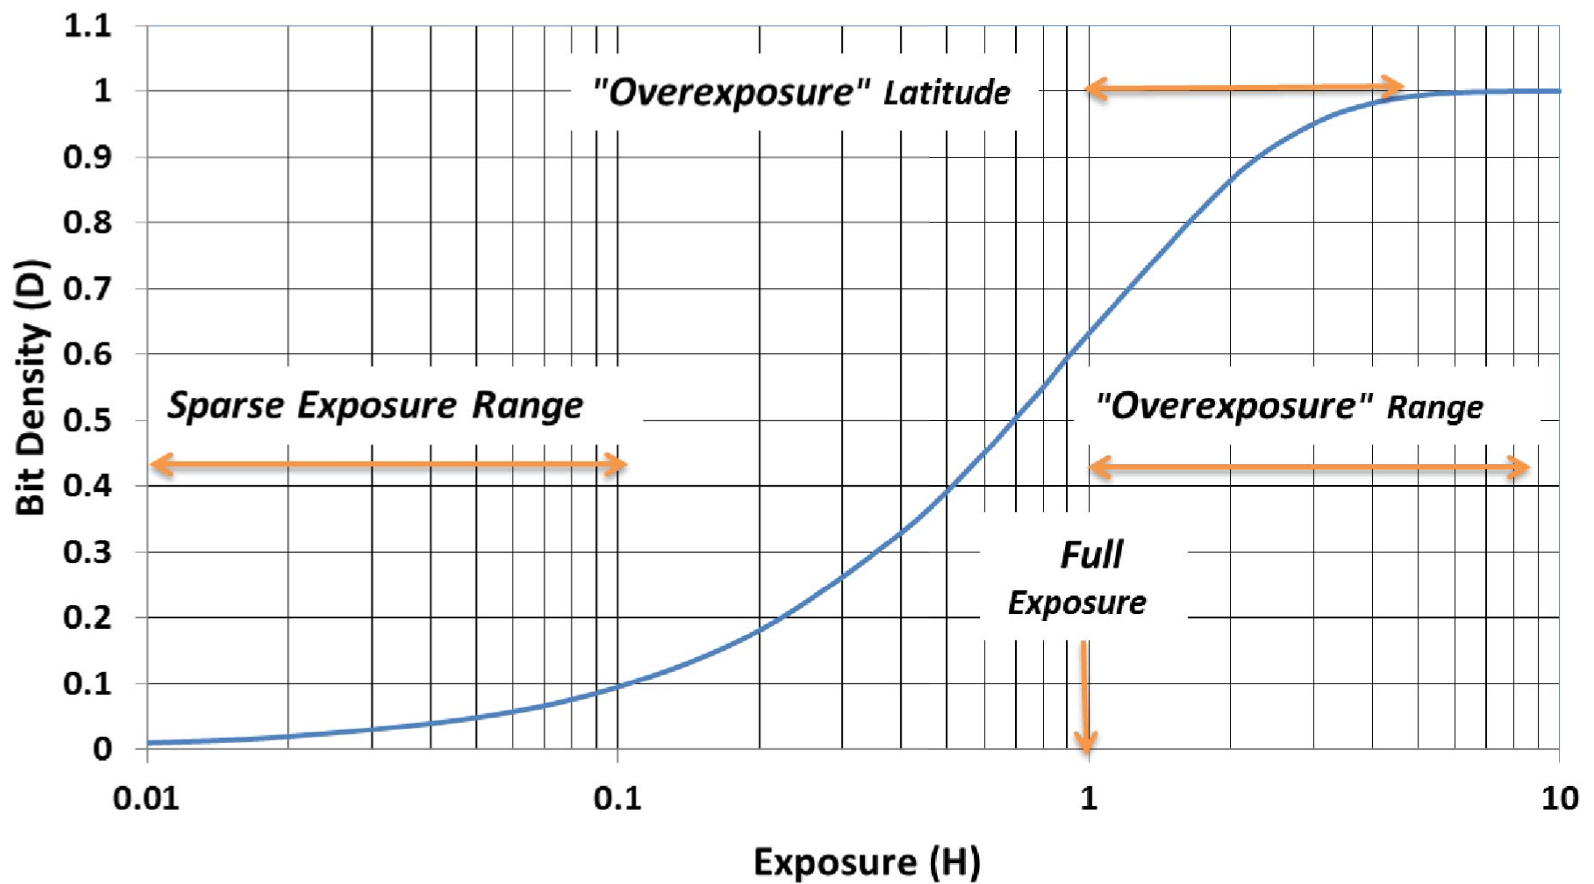
\includegraphics[width=\linewidth]{imgs/film/qiscurve.png}
  \caption{Characteristic curve of the quanta imaging sensor, via \cite{fossum2016quanta}.}
  \label{fig:qiscurve}
  \Description{Shown is the response of the QIS with the S-shaped curve relating the bit density to the exposure.}
\end{figure}


\subsection{SPAD Matrices}

The binary response of the sensor defines the need for a subsequent signal amplification process to generate a sufficiently large voltage signal from a single photon. In one of the currently available gigapixel imaging technologies, this is achieved via the integration of the \textit{single-photon avalanche diode} (SPAD) structures, which implement gain mechanisms internally (\cite{Saleh1991}); this internal amplification process is referred to as electron \textit{avalanche multiplication}~\cite{Ma:17}. Since each detected photon is converted into a cascade of moving carrier pairs, even weak light can produce a clearly detectable current. %The depletion-layer electric field in a photodiode is increased by applying a sufficiently reverse bias across the junction so that the electrons and holes generated may acquire sufficient energy to liberate more electrons and holes within this layer by a process of impact ionization. \cite{Saleh1991} 

\begin{figure}[h]
  \centering
  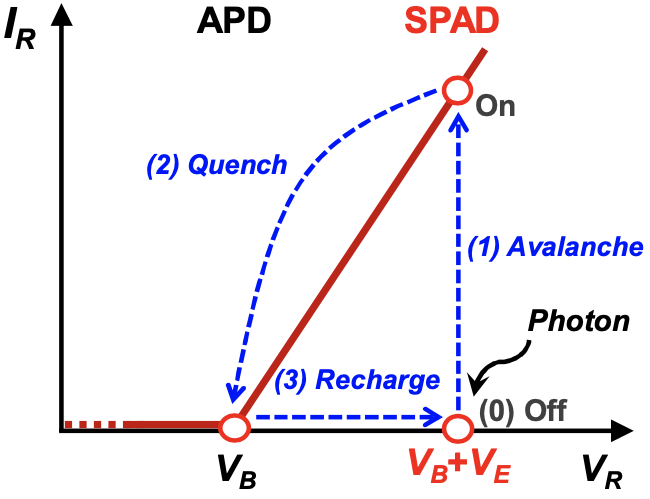
\includegraphics[width=0.8\linewidth]{imgs/spad/avalanche.png}
  \caption{SPAD operation process, demonstrating changes in voltage during the avalanche effect and subsequent quenching. Via \cite{Charbon2018}}
  \label{fig:avalanche}
  \Description{A diagram shows the shift in current during the SPAD-based acquisition process, which happens rapidly for a single photon. Later, the current must drop via quenching.}
\end{figure}

In avalanche photodiodes, the junction electric field is large enough such that the available carriers are accelerated, causing \textit{impact ionization}, i.e., producing further photoelectrons through collision. Ergo, high electrical voltage over 20V is required~\cite{Gnanasambandam_2019}; some prototypes, like the one described in \cite{rng16}, define even higher supply voltages of ca. 22–27V for biasing above breakdown. SPAD is operated in Geiger mode \cite{7117471}. For SPAD arrays, higher breakdown voltage is desirable in general, as it allows for higher photon detection efficiency and improved timing resolution~\cite{7117471}.

The first proposal for a fully integrated CMOS SPAD array has been reported in \cite{Rochas2003}. \cite{DuttonSPAD} allude to other SPAD detectors which have been developed since, noting the variety in both general form (single-point detectors, line sensors, large array photomultipliers, and image sensors) and pixel designs; subsequently, it is stated that no single SPAD-based pixel architecture has been deemed dominant to date. 

The fast detection times in SPADs are associated with the rapidity of the impact ionization process. However, each photon detection event must be followed by finite recovery time, in which the diode is restored to the operative level voltage-wise, freeing excess charge carriers. This process is called \textit{quenching}. During this time, device does not respond to further incident photons. To enable quenching, additional in-pixel circuitry is needed.
Due top the larger amount of transistors needed per single photodetector, the fill-factor of SPAD-based pixels is limited (<40\%), and so is the quantum efficiency (<30\%)~\cite{Ma:17}.

Generally, the SPAD devices aren't entirely compatible with the CMOS technologies due to high operating voltage requirements; the necessity for a large electric field and additional readout circuitry results in the larger dimensions of the structure, lower spatial resolution and higher power dissipation~\cite{Ma:17}. Furthermore, the generation of electrons is based on thermal reactions, rendering the detectors significantly more susceptible to dark current.

However, significant progress has been achieved in recent years~\cite{SPADperformance, rng16}. Performance of SPAD-based architecture using the developments in 3D stacking technologies is described in detail in \cite{Charbon2018}.



\subsection{The Pixels as Jots}

The avalanche-mode operation in SPAD-based photodetectors limits the pixel pitch and the manufacturing yield and delivers highly undesirable amounts of dark current, which can be somewhat reduced through cooling. In fact, the abstinence from the avalanche photodiode technology is stated to be one of the design criteria in photon-counting applications.
Quanta imaging sensor (or QIS for short), a different implementation of the binary image sensor, attempts to overcome such limitations\cite{Ma:17, Ma03rmsJot}.
The principal advantages of CMOS arrays (low-voltage operation, low power consumption, ease of integration of on-chip operation control, the possibility of random access to the image data, etc., \cite{Holst2011}) must be retained. %S.105

In QIS, the photodetectors are intentionally made small as to be capable of storing charges of several electrons. 
Placed together in a structure, these become \textit{jot devices}, with "jot" denoting the ``smallest thing'', a word of Greek origin \cite{FossumSiMulQIS}.

In some of the available research (\cite{s16111961}), jots are referred to as subpixels, or, partitions of conventional CMOS memory bit-cells; other sources (\cite{fossum2016quanta}) may use the term ``\textit{SDL pixels}'', referring to the pitch values within sub-diffraction limit (200-500$n$m).

The jot photoelements have a \textit{small full-well capacity} (FWC, or storage capacity density, often provided in photoelectrons per cm$^2$), which ranges from one to around 100 or 200 carriers -- compared with the state-of-the-art conventional imaging sensors where the full well is first reached at ca. 4000$e^{-}$~\cite{Gnanasambandam_2020}, the values are low. Subsequent circuitry discriminates the output to one of the binary states \cite{FossumSiMulQIS}, based on the pre-defined, semi-arbitrarily set threshold $q$. 

Instead of converting the number of photons impinging on the sensor surface to voltage, either 1 or 0 are transferred and quantized. Precision of quantization is not of essence. The thresholds are set lower due to the relatively small FWC, and the binary response is triggered quickly. Thus, unlike conventional CIS pixels (described as "buckets" accumulating and integrating [larger] charges of multiple photoelectrons), jots require lesser integration times and can be readout at rates as high as 1000 frames, or fields, per second. 

\cite{MaJotDevices} envision QIS to have structures consisting of 0.1...10.0 Gjots; due to the fast readout speeds, dimensions of this order must lead to data rates of 0.1...10 Tb/s.

Research regarding the quanta imaging sensor technology is currently in progress. A prototype of camera featuring QIS has already been produced, albeit with a lesser spatial resolution and pixel pitch than sought-after. Representing a crucial paradigm shift, this imaging technology has full potential to stand in as the third generation of digital sensors, replacing CMOS. The benefits, advantages, and the detailed methodology behind QIS will be discussed in the remainder of this paper.

\section{Quanta Imaging Sensor}
\subsubsection{Jot Data Structure}
%Frames readout off the sensor are accounted for during the image formation, allowing for estimation of the local light intensities as a function of time.

\begin{figure}[h]
  \centering
  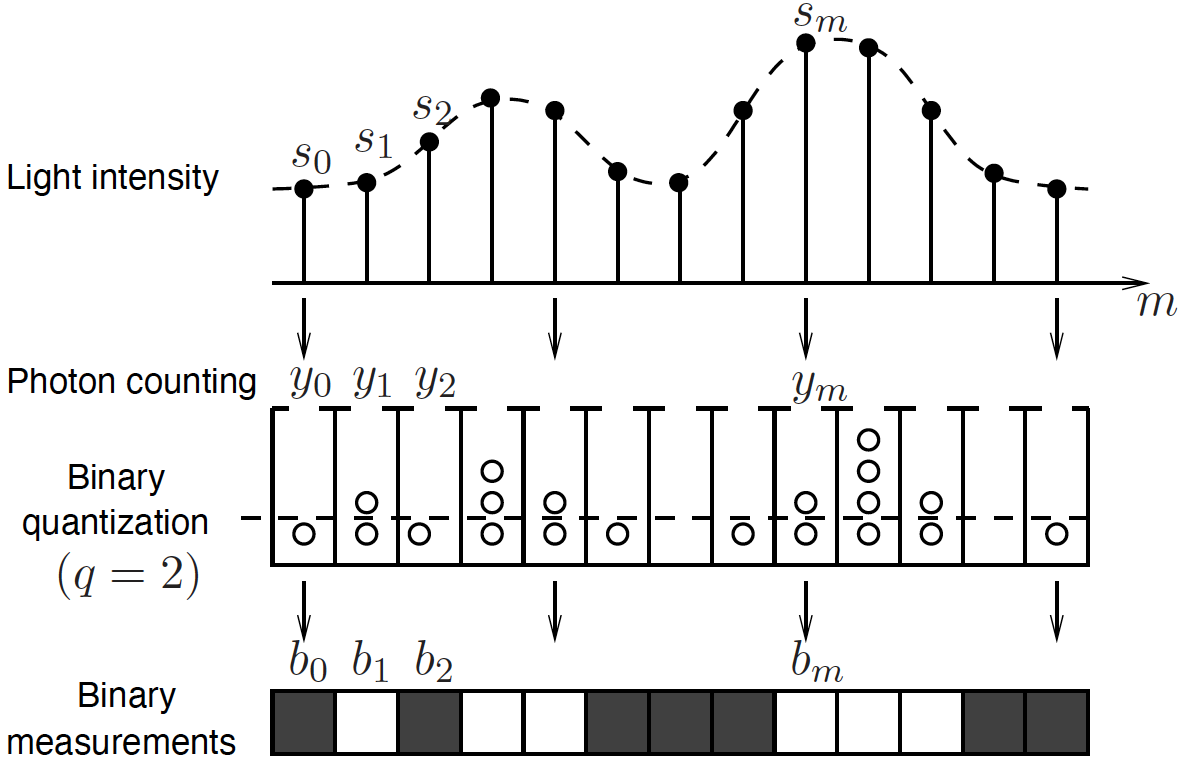
\includegraphics[width=\linewidth]{imgs/sensors/binarysensor.png}
  \caption{Binary sensor model, via \cite{Feng_Yang_2012}.}
  \Description{Photon-counting process in an oversampled binary sensor.}
\end{figure}

The output of the simple QIS design is binary in nature. Combined output of the QIS jots is a series of bit planes, observed over time. Since both spatial and temporal sampling take place, the output can be conceptualized as a cube, as shown in Figure \ref{fig:jotcube}.

\begin{figure}[h]
  \centering
  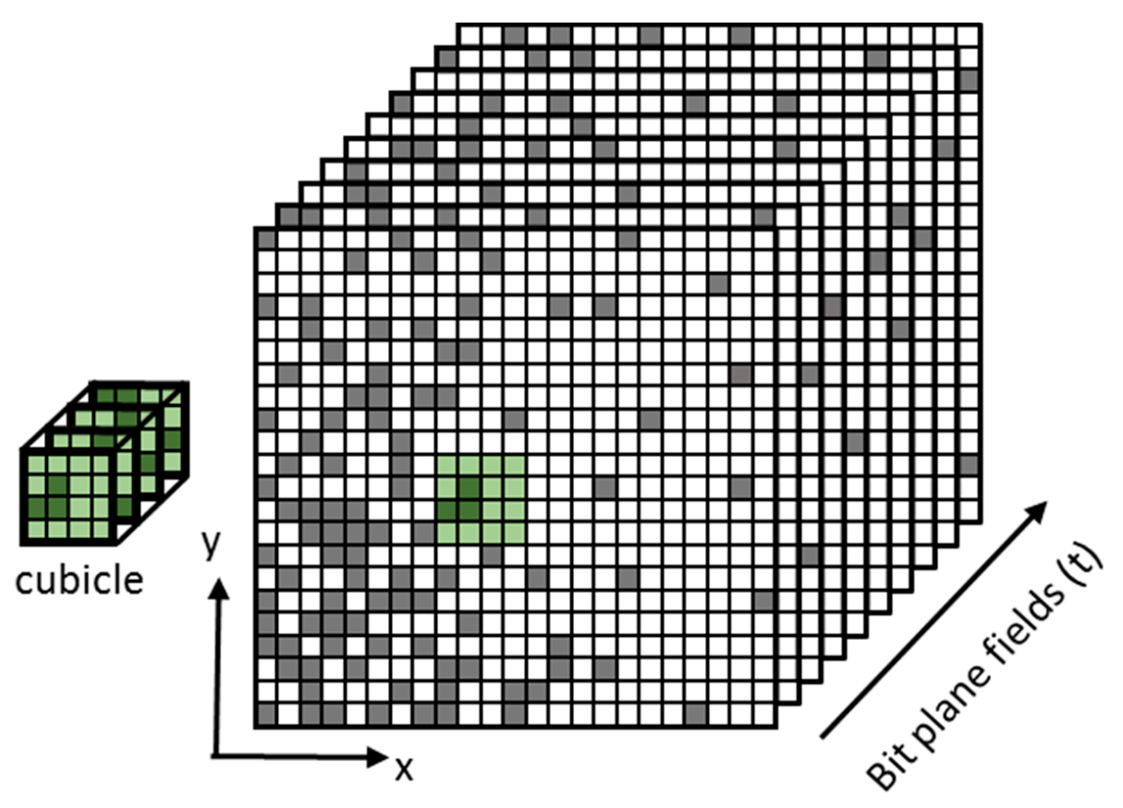
\includegraphics[width=0.7\linewidth]{imgs/qis/jotdatacube.png}
  \caption{Jot data cube, via \cite{fossum2016quanta}}
  \label{fig:jotcube}
  \Description{The output of a quanta image sensor, divided into binary values corresponsing to the spatial $x$-$y$-coordinates and the temporal dimension $t$.}
\end{figure}

Unlike CIS arrays which produce images of fixed sizes, quanta imaging sensor allows the output pixel image size to be programmable and dynamically adjustable~\cite{FossumSiMulQIS}; the image reconstruction mostly occurs post-acquisition, and the bit plane can be divided into smaller jot cubicles of arbitrary sizes which should then form a single pixel in the conventional sense from temporal and spatial data.

It is understood that the forming of the image pixels does not require uniformly sized jot cubicles; for separate pixels, these can have different dimensions in $x$, $y$, and $t$. It follows that selected cubicles of the adjacent pixels may overlap, aiding formation of multiple CIS pixels at once~\cite{fossum2016quanta}.

\subsection{Distinctions}

The similarity of the QIS response to the sensitivity of the photographic film emulsion has been established in the previous sections; in both cases, the shape of the characteristic curve is determined by the photon arrival statictics. 

In film, around 3-4 carriers were needed to elicit the chemical reaction. Since the binary value is obtained through comparisons against a certain threshold, the choice of threshold can influence the final response. Figure \ref{fig:qiskt} shows the response curves plotted for the number of carriers $k_{T}$ needed for the single-bit pixel output of ``1'' ($k_{T}=1,2,3,4,20$). It is evident that the linearity of the QIS response curve changes with the larger thresholds; similarly, the overexposure latitude is shifted towards larger exposures. Hence, the single-bit jot devices can be applicable under multiple varying lighting conditions, enabling low-light and high dynamic range imaging applications, where the acqusition using multiple threshold values would provide different values for linearity.

\begin{figure}[h]
  \centering
  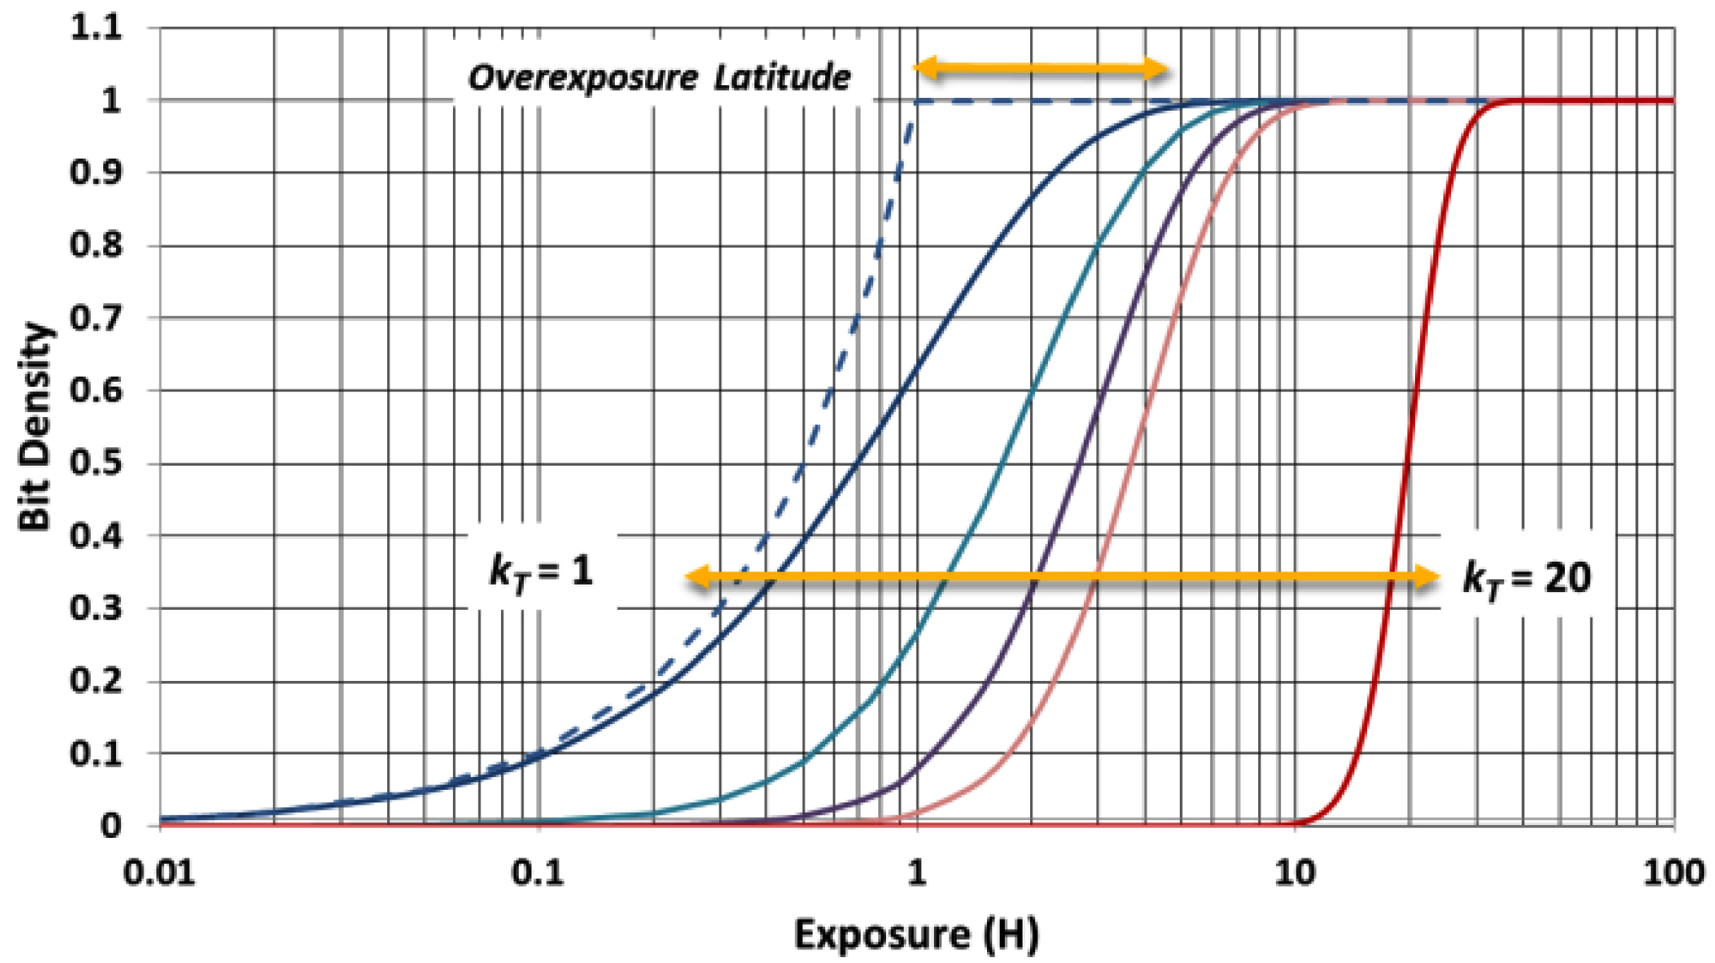
\includegraphics[width=\linewidth]{imgs/qis/multicarrier.png}
  \caption{Single-bit QIS response curves in dependence of the amount of carriers, via \cite{FossumSiMulQIS}}
  \label{fig:qiskt}
  \Description{Response curves of QIS depending on the threshold. For larger values, the slopes are narrower, and the overexposure latitudes are reached upon stronger illumination, albeit more quickly.}
\end{figure}

For this reason, it is convenient to distinguish between the single-bit jot devices with full-well capacitances in the classical sense, of only one electron (\textit{single-carrier}), and multiple electrons (\textit{multi-carrier}) which can be dynamically adjusted in their responses based on the threshold.

\subsection{Hardware Design}

To facilitate the transition to the QIS as the future dominant sensor technology in the future, strong compatibility with a CIS fabrication line must persist.

CMOS sensor serves as a suitable basis for quanta imaging due to its low voltage specifications, high quantum efficiency, high spatial resolution, and more. \cite{Ma:17}. 
However, due to the source-follower output voltage, the read noise is too high to enable photon detection. Current state-of-the-art CIS demonstrate read noise in the ranges of 1...2$e^{-}$ r.m.s. ~\cite{7273747}. Due to the binary nature of the signal, such amount of noise has grave consequences for the single-bit QIS, resulting in high possibilities of false misquantization. At low light levels, desired read noise in single-bit QIS should amount to 0.3$e^{-}$ r.m.s. at best, delivering error-free estimation with 0.15$e^{-}$ r.m.s. under especially sparse exposures (0.01<H<1). For such low bit error rates, conversion gain of at least ca. 1$m$V/$e^{-}$ is needed, which is five times higher than the values demonstrated in the state-of-the-art CIS devices~\cite{MaJotDevices}.
For this reason, current CIS technologies must be modified in order to enable photon-counting.

%Instead of using avalanche gain to detect single photoelectrons, the gain comes from using a very small sense node capacitance yielding CG in the range of 500uV/e-. Using intrapixel charge transfer, a single electron transferred to that capacitance can produce a signal that is well above the noise floor (e.g. 0.2e- rms noise floor) and thus give a low error rate for detection of single photoelectrons. The detection process is slower than for SPADs, but sub-microsecond timing is achievable. Further, avoiding the high electric fields of SPADs enables smaller pixels or jots, improved manufacturability, and thus lower cost per pixel and smaller optics. Power dissipation is also considerably smaller. In late 2017, Dartmouth reported a 1Mpixel QIS device implemented in a nearly standard CMOS BSI stacked process with 1.1um pixel pitch, operating at 1000fps and dissipating about 20mW total power. The 1Mpixel QIS was demonstrated more than two years earlier than the 1Mpixel SPAD array and with much less development time and with much smaller pixels. About 73 CMOS QIS pixels can fit into the area of one SPAD pixel. This is the strength of working in nearly standard CMOS image sensor processes. The applications of QIS are currently being explored but include low-light imaging for security, defense and science.
%\cite{9059308}

%Single jot is described having storage well of 1...200$e^{-}$. 
During the charge-to-voltage conversion, the signal transfer is corrupted by noise  due to the voltage fluctuations and the parasitic capacitances in the circuitry, which reduce the transfer efficiency. %may end up corrupted by noise 
Higher conversion gain ensures that the estimations are accurate, and the transferred electrons are capable of producing signal above the noise floor. This could be achieved by increasing the voltage, however, higher operating voltage would render the sensor incompatible with most baseline CMOS processes.\cite{Ma:17} Otherwise, one can attempt to minimize the read noise, which is caused by the capacitance of the floating diffusion. In available works, FD is minimized via specialized jot structures, where the doping profiles of the pixels are modified via implantations.
Jot candidates based on their doping properties are covered in detail \cite{Masoodian16, Ma:17}. On average, the doping profiles of the jots have lead to the reduction of the noise to ca. 0.21$e^{-}$ r.m.s. with the conversion gain nearing 350$\mu$V/$e^{-}$ with 15\% variation~\cite{Ma:17}.

Most of the publications referenced in this work explore prototypes for jot devices which were fabricated in conformance with the 45/65nm 3D stacked CMOS process with backside-illumination (BSI), which guarantees high fill factor and quantum efficiency~\cite{Ma03rmsJot}.

Figure \ref{fig:qischip} demonstrates the architecture of existing 1Mjot clusters with vertical integration. The jot device is vertically separated from the readout circuitry, which reduces the total area and allows faster readout. Presented array can be implemented with analog and digital readout circuitry; Such clusters can be arranged in parallel, thus forming a chip of significantly larger dimensions without any significant delays in speed. In this particular jot device, analog clusters were integrated together with the digital clusters.

%Above all, in order to achieve the theorized performance, the jots must achieve higher conversion gain, and the appropriate architecture for the binary analog-to-digital-converter must be found to ensure that the resulting read noise is in the deep sub-electron range.

%Quanta imaging sensor inherits CIS advantages in terms of pixel size, spatial resolution, dark current, quantum efficiency (QE), readout speed, and power dissipation. Beyond CIS and existing photon-counting technologies, the QIS aims to realize accurate photon counting without avalanche gain or cooling, while maintaining low dark current and manufacturing cost.\cite{Ma:17}

\begin{figure}[h]
  \centering
  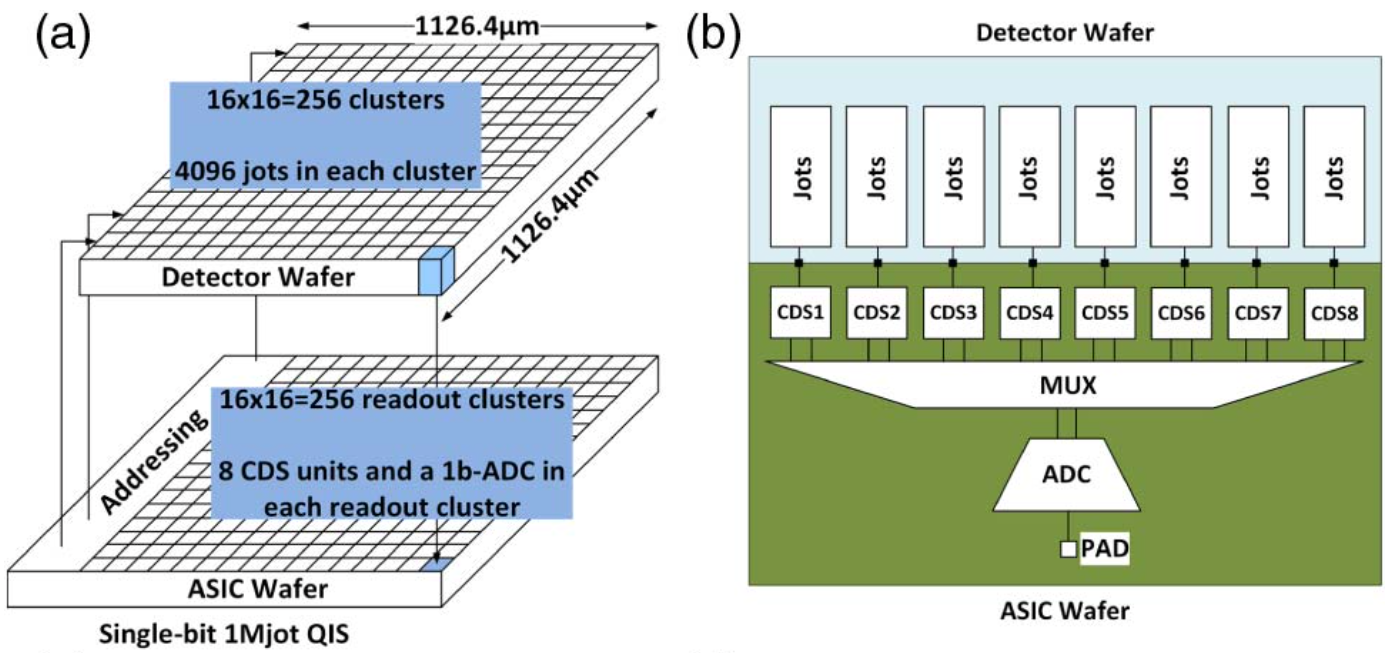
\includegraphics[width=\linewidth]{imgs/qis/mjot-wafer.png}
  \caption{Simplified architecture of the 1 Mjot stacking QIS chip (left) and one digital cluster (right), via \cite{Ma:17}}
  \label{fig:qischip}
  \Description{The wafer containing the photodetectors is positioned vertically above the circuitry. The jots are united in clusters, each cluster has a designated circuitry unit for readout.}
\end{figure}

\begin{figure}[h]
  \centering
  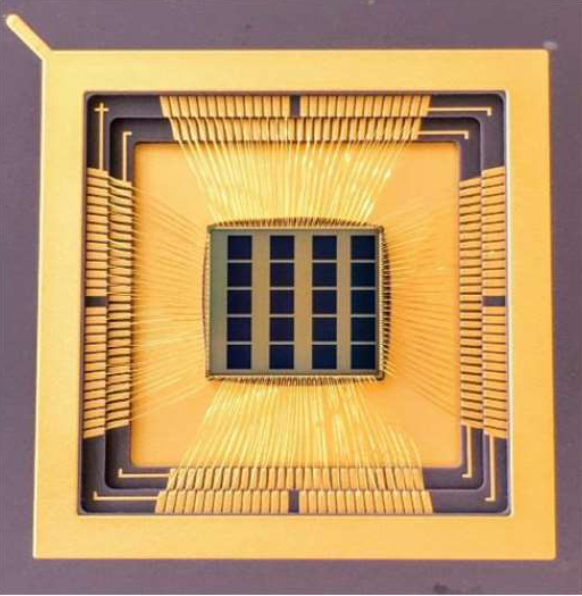
\includegraphics[width=0.5\linewidth]{imgs/qis/20Mjot.png}
  \caption{QIS test chip featuring 20 1Mjot arrays (left), via \cite{s19245459}.}
  \label{fig:20mjots}
  \Description{Yellow sensor chip realizing 20 Mjot clusters. The clusters are placed in a grid on the sensor plane.}
\end{figure}

Within a single-bit QIS, ADC acts as a simple comparator with an exposure-appropriate threshold $q$. Since the response is binary, the bit depth of only 1 is required for quantization.

\subsection{Multi-Bit QIS}

The field readout rate of the sensor can be traded off for the increased bit depth of the ADC, thus allowing to count more photoelectrons per each readout cycle. Such implementation of the sensor, the multi-bit QIS, can be seen as the middle ground between the conventional CIS and the single-bit photon-counting sensor~\cite{ADCmultibit}. The carrier numbers, which were previously reduced to single-bit values, can now be mapped to their respective quantities in a certain range. Upon saturation, the maximum number of the converter is reported instead~\cite{FossumSiMulQIS}.

Through lowered framerates and increased electron resolution, the output data transfer rate can be lowered. The increase in complexity of the ADC is negligible in comparison with the lowered complexity of the calculations; since the represented number of carriers is defined to be in the range of 1...200$e^{-}$, the resolution of the ADC does not need to be overly high, presenting significant improvements with the bit depth of $n = 6$. Reduction of the framerate for a multi-bit QIS occurs by the factor $2^n -1$; assuming the framerate of 1000 fps for single-bit QIS, the framerate of a multi-bit QIS will amount to $\frac{1000 \textup{fps}}{2^{n}-1}$, ensuring reduction by the factor of 63 in case with the 6b ADC.

Another advantage provided by the bit depth selection is the ability to adjust linearity and compression between the input photon flux and the output signal.

The prototype in Figure \ref{fig:20mjots} features 20 1Mjot arrays, allowing easy and flexible scaling in overall resolution due to the cluster-parallel architecture mentioned earlier. However, with each integrated arrays, the power dissipation is multiplied accordingly. The choice of ADC architecture for multi-bit QIS in terms of power consumption has been evaluated in \cite{ADCmultibit}, where the successive approximation register ADCs were deemed too be the least power-consuming option in relation to the occupied area. 


\subsubsection{Color Imaging}

Spectral information in digital sensors is typically obtained using \textit{color filter arrays} (CFAs), semi-transparent masks integrated on top of the sensor. These form a 2D periodical pattern with the three primary colors. Thus, each pixel is limited to irradiance related to the wavelength range of the respective color.

Later, the intensity values in each 2D kernel are reconstructed and interpolated, or \textit{demosaicked}, to form a single pixel with three colour channels.

The most widely used CFA configuration is Bayer RGB pattern, though many other arrangements exist~\cite{Krig2014}. Figure \ref{fig:cfabayer} shows the Bayer pattern and its exemplary position on a sensor plane.

\begin{figure}[h]
  \centering
  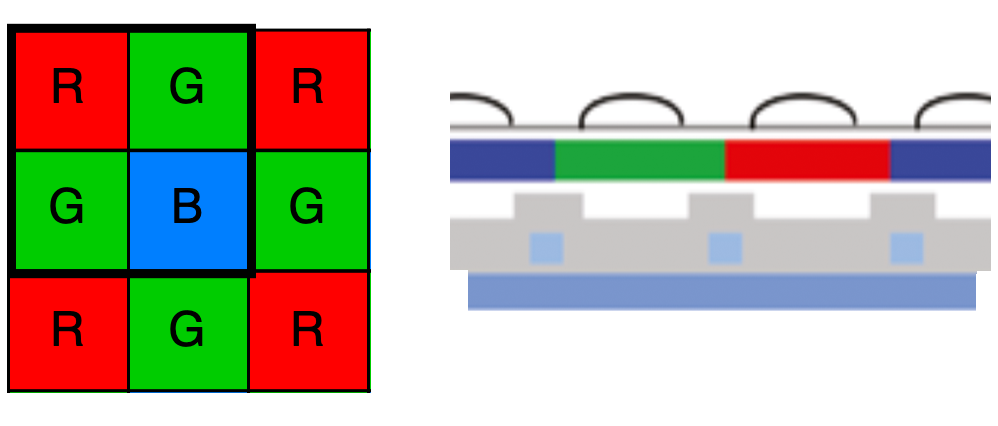
\includegraphics[width=0.8\linewidth]{imgs/cfabayer.png}
  \caption{Bayer RGB pattern and the common integrated CFA arrangement (right, via \cite{Krig2014}).}
  \label{fig:cfabayer}
  \Description{Pattern of Red, Green, Green, Blue is placed on top of the electronics.}
\end{figure}

Following problems pertain through inclusion of color information via CFA:

\begin{itemize}

\item \textbf{Aliasing}. Through demosaicking, combined spatial resolution is lowered, and under sampling rates below the Nyquist frequency, \textit{Moiré artifacts} appear.

\item \textbf{Reduced sensor sensitivity}. Part of light is blocked out and never reaches the sensor plane, and the net signal is more susceptible to noise.

\item \textbf{Crosstalk}. The optical or electrical charge in the pixels may leak towards the adjacent pixels. In CFAs, where charges depend on wavelengths and change rapidly, this results in a desaturation of the color measurements.
\end{itemize}

While these problems appear in monochromatic sensors as well, here, the errors persisting translate to false color values, which is more disturbing for the human perception \cite{Hunt2005}.

Not all effects are equally pronounced, however, attempts to alleviate one factor may result in higher impact of the others. For one, QIS sensors are unaffected by aliasing due to their small feature sizes, while conventional CMOS sensors may require designated algorithmic suppression. At the same time, smaller pixel pitches lead to severe crosstalk; even more so when the adjacent colors are different~\cite{elgendy2019color}, which is the case with the Bayer pattern. In binary sensors, the leakage means false positives, resulting in a substantially lower SNR.

\cite{Anzagira2015ColorFA} attempt to mitigate the crosstalk through the extensions of Bayer pattern. 

\begin{figure}[h]
  \centering
  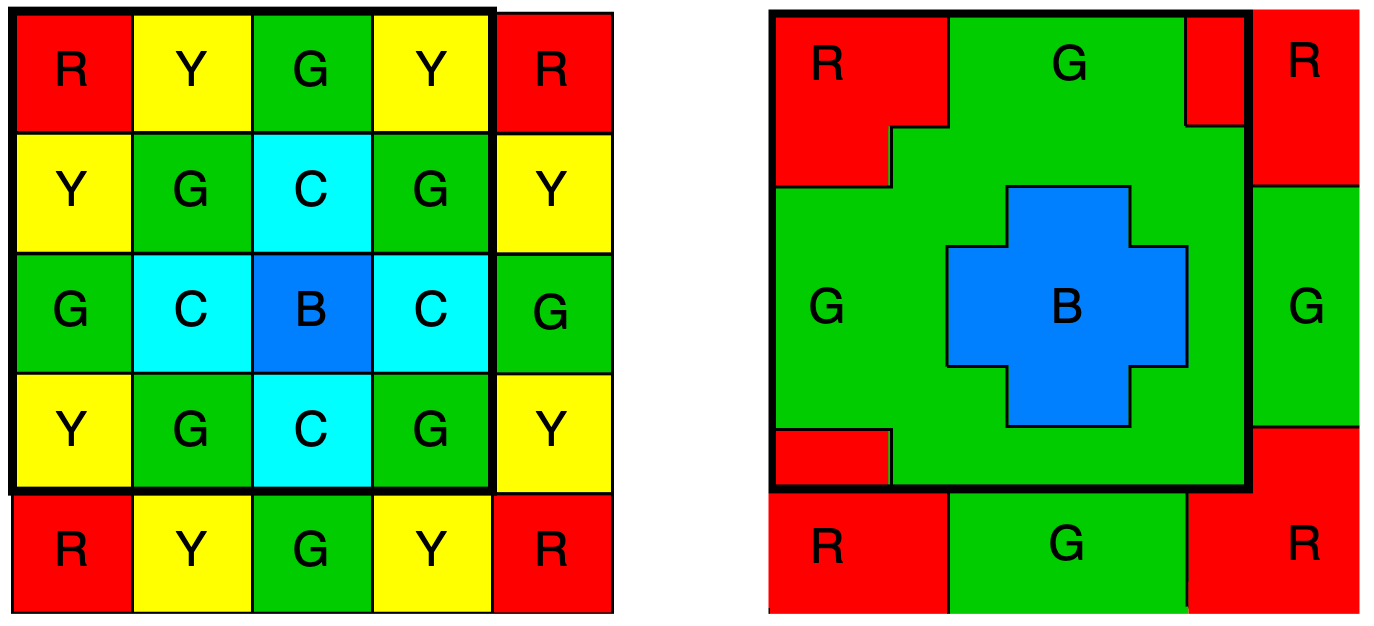
\includegraphics[width=0.7\linewidth]{imgs/cfaqis.png}
  \caption{CFA Proposals made in \cite{Anzagira2015ColorFA}.}
  \label{fig:cfaqis}
  \Description{Squared patterns for color imaging, which now include more secondary colors in the arrays or the larger bounds of the primary colors in the pattern masks.}
\end{figure}

Figure \ref{fig:cfaqis} depicts two of the proposals. On the left, the initial mosaic is expanded through secondary colors cyan, magenta, and yellow. These are positioned between the respective primary colours so that the spectral overlap is smaller. For increased light sensitivity, some of the green pixels may also be replaced with white. The second proposal expands the active color regions of the filter, leveraging the high spatial resolution of the QIS. The overlaps now occur in the regions where the pixels are halved, which can be accounted for during computations.

%Assume cross-talk to be equal for all wavelengths and only pertain in vertical and horizontal directions

\cite{elgendy2019color} focus on more than merely crosstalk mitigation, proposing design criteria for sub-diffraction limit CFAs.
Paired with a demosaicing algorithm, this should maximize spatial resolution between the channels while improving the sensitivity in general. Similarly, the demosaicking process should minimize the noise power after the light passes the filter. 

Presented in Figure \ref{fig:cfaelgendy}, the filter has a diagonal structure. The auxiliary demosaicking algorithm works on frequency selection and was found to be universally applicable, performing well in both CIS and QIS imagers.

\begin{figure}[h]
  \centering
  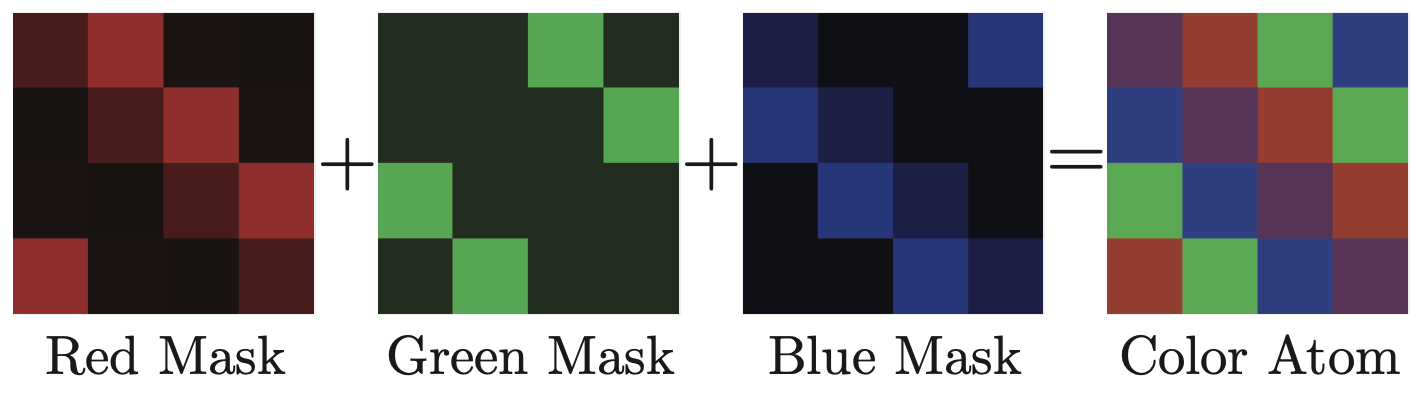
\includegraphics[width=0.7\linewidth]{imgs/cfaelgendy.png}
  \caption{CFA pattern proposed in \cite{elgendy2019color}. The patterns are positioned diagonally, with gradations, as to reduce the cross-talk between the pixels.}
  \label{fig:cfaelgendy}
  \Description{Primary colors in the pattern are positioned diagonally}
\end{figure}

In both cases, the filter kernel is larger, and the spatial resolution of the sensor is traded off for better performance in presence of crosstalk. 


 \begin{figure}[h]
  \centering
  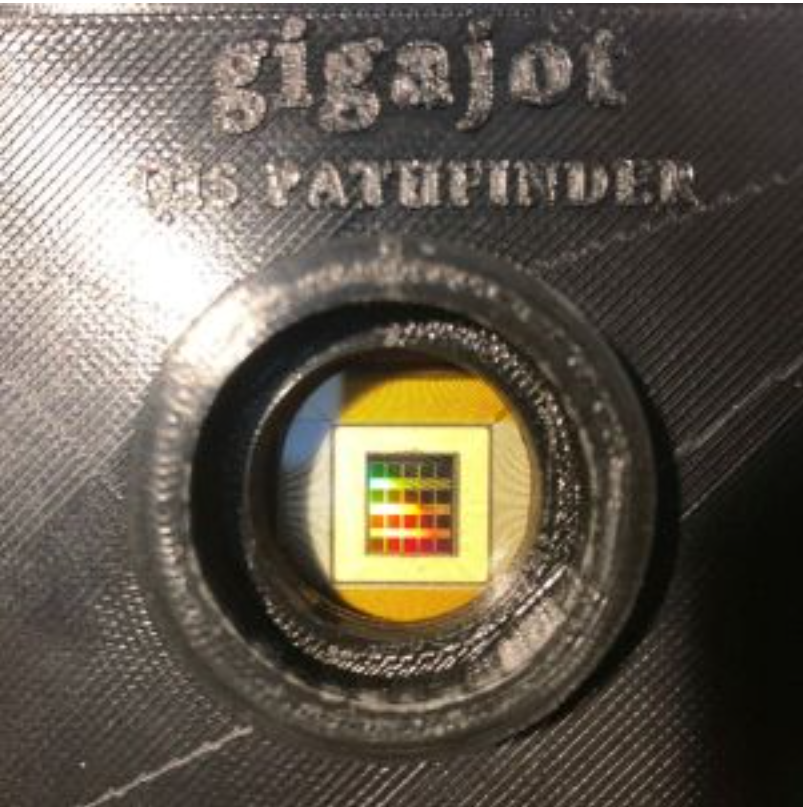
\includegraphics[width=0.5\linewidth]{imgs/qis/gigajot.png}
  \caption{Quanta imaging sensor, as seen in a Gigajot camera. Via: \cite{Gnanasambandam_2019}}
  \Description{Small industrial camera with equally small lens above it}
\end{figure}

The strictly algorithmic processing of the color image in QIS has been described and applied in \cite{Gnanasambandam_2019}, who present the QIS Pathfinder camera module developed at Gigajot Technology with a Bayer pattern color filter array implemented on-chip. 


\subsection{Compared Performance}

Table \ref{tab:comp} shows some of the most significant operating parameters for the two photon-counting sensor implementations. We have collected these specifications based on the state-of-the-art implementations of the devices reported in the references section, taking the values from the most recently published sources in case of ambiguities.

It is evident that while SPAD-based arrays have higher dark current through thermally-induced avalanche gain, their read noise is still rather low, and the framerate is higher than the one in QIS by several orders of magnitude. The reasons for this behavior, i.e. the amount of circuitry required to implement quenching, were mentioned in detail in previous sections. The read noise in QIS is nearing the ideal, relatively error-free value of 0.15$e^{-}$ r.m.s., while the dark current is completely negligible.

\begin{table}
  \caption{Comparison of QIS and SPADs}
  \label{tab:comp}
  \begin{tabular}{l|cc}
    \toprule
    Parameters & QIS & SPAD\\
    \midrule
    Pixel pitch & 1.1$\mu$m & 5-10$\mu$m\\
    Read noise [RT] & 0.21$e^{-}$ r.m.s. & <0.15$e^{-}$ r.m.s.\\
    Dark current [RT] & 0.16$e^{-}$ r.m.s. & >10$e^{-}$ r.m.s.\\
    Framerate & 1040 fps & 97 000 fps \\
    Quantum efficiency & 70-80\%  & 30-50\% \\
    Fill factor & >90\% & <70\% \\
    Full well capacity & 1-200$e^{-}$ & N/A \\
    Operating voltage & 2.5/3.3V & 15-25V\\
    \bottomrule
  \end{tabular}
\end{table}

The contrast in approaches is noticeable in almost every other specification. Compared to QIS, SPADs need high electrical voltage to accelerate the photoelectrons, while providing lesser quantum efficiency. Such differences provide a clear distinction between the applications of both photon-counting sensors: SPAD-based imaging is significantly more functional in applications that value acquisition rate above all and need better temporal resolution, e.g. Time-of-Flight imaging, while QIS is better suitable for applications that prioritize accuracy and low-light sensitivity. Low-light imaging applications of QIS may include astronomy, surveillance, medical examinations, and many others. With sufficiently large oversampling, the single-bit QIS can have substantially higher dynamic ranges, being able to acquire scenes containing both bright and dark regions~\cite{Feng_Yang_2012} and benefitting from the non-linear binary curve. According to \cite{9059308}, about 73 CMOS QIS pixels can fit into the area of one SPAD pixel, rendering the technology especially desirable in microbiology purposes.